%\documentclass{beamer}
\documentclass[10pt]{beamer} 

\usepackage[utf8x]{inputenc}
\usepackage{amsmath,amsfonts,amssymb}
\usepackage{verbatim} 
\usepackage{graphicx}
\usepackage{color}
\usepackage{multimedia} 

\usetheme{Frankfurt}
\usefonttheme{professionalfonts}



\setbeamercovered{transparent}

\title[Motion generation with GPDM and Inverse Kinematics]{Motion generation with GPDM and Inverse Kinematics}
\subtitle{Lab Talk}

\author[N. Taubert]{Nick Taubert}

\date[22.02.12]{22. February 2012}

\begin{document}

\begin{frame}
  \titlepage
\end{frame}

\begin{frame}
  \frametitle{Outline}
  \tableofcontents[pausesections]
\end{frame}

\section{Introduction}
\subsection{Gaussian Process Latent Variable Model}
\begin{frame}
  \frametitle{Gaussian Process Latent Variable Model}
  \begin{columns}[c]
    \column{4.9cm}
	\tiny{\hspace{1cm}$N\mathop{\hat{=}}$ length of the dataset

	\hspace{1cm}$D\mathop{\hat{=}}$ dimension of the dataset

	\hspace{1cm}$q\mathop{\hat{=}}$ dimension of the latent space}
    \column{5cm}
	\includegraphics<1-2>[height=3.3cm]{./Images/GP_LVM_01.eps}
	\includegraphics<3>[height=3.3cm]{./Images/GP_LVM_GP01.eps}
	\includegraphics<4-6>[height=3.3cm]{./Images/GP_LVM_GP02.eps}
	\includegraphics<7-8>[height=3.3cm]{./Images/GP_LVMall.eps}
    \column{5cm}
      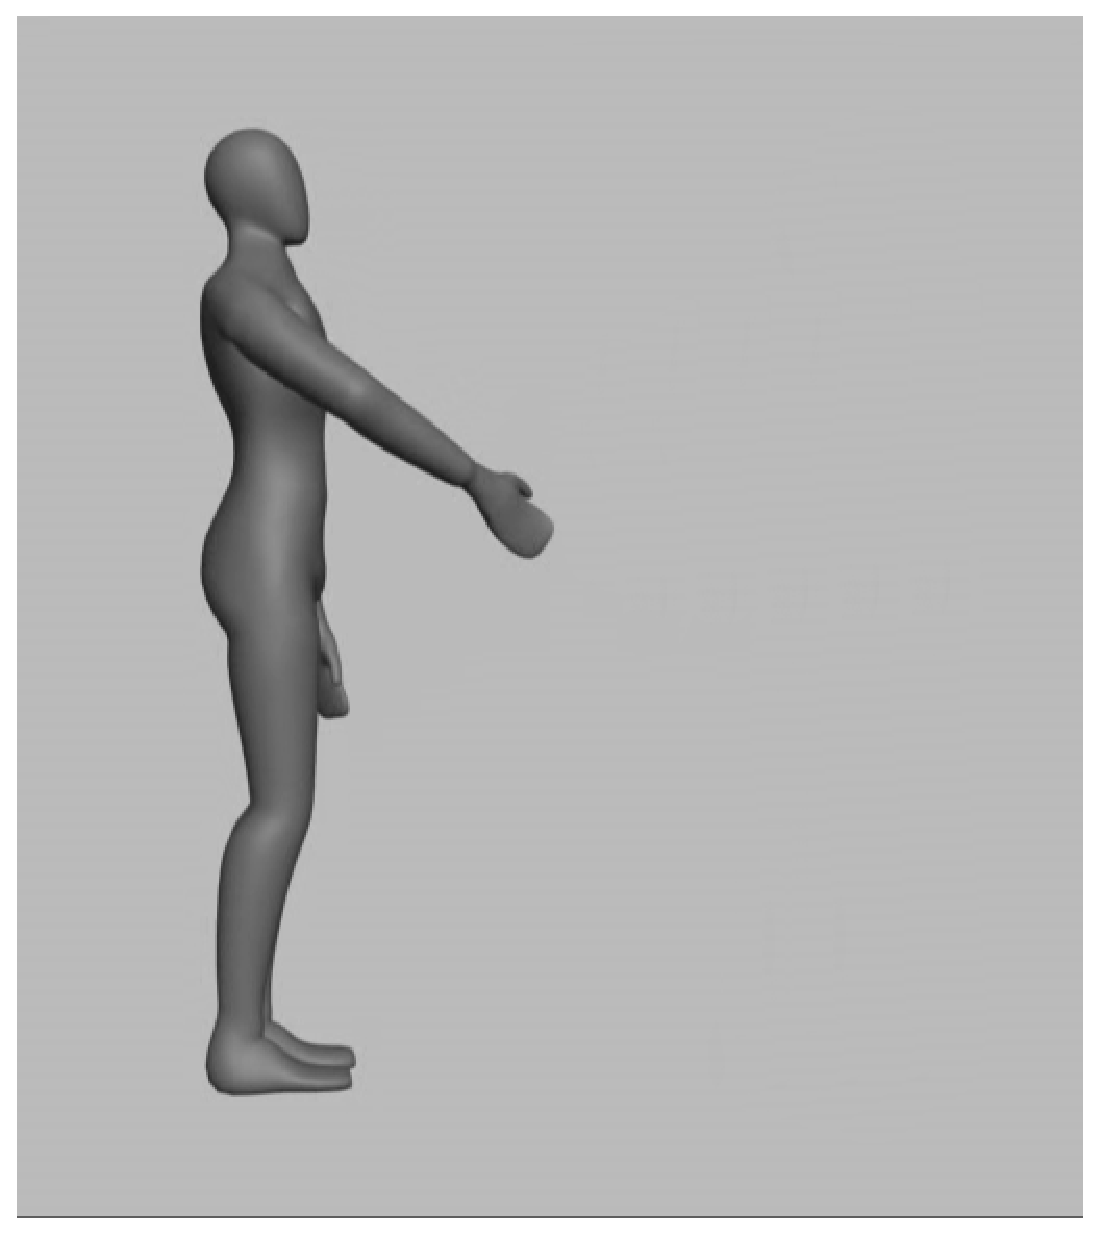
\includegraphics[height=2cm]{./Images/NaturalHandshakes_GPsingle.eps}
  \end{columns}
  \vspace{20px}
  \begin{overlayarea}{\textwidth}{5cm}
      \only<1>{
	\begin{itemize}
	  \item An actor is represented by a Gaussian Process Latent Variable Model (GP-LVM),
	  \item a high dimensional dataset $\mathbf{Y}=[\mathbf{y}_1,...,\mathbf{y}_N]^T$ $\in\Re^{N\times D}$ ($D=114$) were represented
	    through a low dimensional latent variable $\mathbf{X}=[\mathbf{x}_1,...,\mathbf{x}_N]^T$ $\in\Re^{N\times q}$ ($q=3$).
	\end{itemize}
      }
      \only<2-4>{
	Gaussian Process is the prior on the mapping from latent space to the data space:
	\uncover<3-4>{\[\mathbf{y} = f(\mathbf{x}) + \varepsilon,\hspace{1cm}} \uncover<4>{f(\mathbf{x})\sim GP(m_Y(\mathbf{x}),k_Y(\mathbf{x},\mathbf{x}'))\]}
      }
      \only<5>{
	For a high dimensional reduction and smooth trajectories in latent space we are using a non-linear rbf kernel in the form of
	\[k_Y(\mathbf{x},\mathbf{x}')=\beta_1\exp\left(-\frac{\beta_2}{2}|\mathbf{x}-\mathbf{x}'|^2 \right)+\beta_3^{-1}\delta_{\mathbf{x},\mathbf{x'}},\]
	which builds the $N\times N$ kernel covariance matrix $\mathbf{K}_Y$.
      }
      \only<6-8>{
	Learning the GP-LVM is then equivalent to minimizing the negative Log-Likelihood of the model:
	\begin{eqnarray*}
	    \mathcal{L} & = & -\ln p(\mathbf{Y}|\mathbf{X},\bar{\beta})\uncover<7-8>{p(\mathbf{X})p(\bar{\beta})} \\
	    \uncover<8>{& = & -\frac{DN}{2}\ln2\pi-\frac{D}{2}\ln|\mathbf{K}_Y|-\frac{1}{2}\mathbf{Y}^T\mathbf{K}_Y^{-1}\mathbf{Y}
	    -\frac{1}{2}\sum_{n=1}^N \mathbf{x}_n \mathbf{x}_n^T-\sum_{j}\ln\beta_j,}
	\end{eqnarray*}
	\uncover<8>{assume: $m(\mathbf{x})=0, \mu=0, \Sigma=I$}
      }
  \end{overlayarea}  
\end{frame}

\subsection{Graphical Model Representation}
\begin{frame}
    \frametitle{Graphical Model Representation}
    \begin{columns}[c]
    \column{4.0cm}
	  \tiny{\hspace{1cm}$N\mathop{\hat{=}}$ length of the dataset

	  \hspace{1cm}$D\mathop{\hat{=}}$ dimension of the dataset

	  \hspace{1cm}$q\mathop{\hat{=}}$ dimension of the latent space}
      \column{5.7cm}
	\includegraphics<1>[height=4.7cm]{./Images/Model_ActorStart.eps}
	\includegraphics<2>[height=4.7cm]{./Images/Model_ActorTrials.eps}
	\includegraphics<3>[height=4.7cm]{./Images/Model_ActorEmotion.eps}
	\includegraphics<4>[height=4.7cm]{./Images/Model_ActorCouple.eps}
	\includegraphics<5>[height=4.7cm]{./Images/Model_InteractionOnly.eps}
	\includegraphics<6>[height=4.7cm]{./Images/Model_Interaction.eps}
	\includegraphics<7>[height=4.7cm]{./Images/Model_HMM.eps}
	\includegraphics<8>[height=4.7cm]{./Images/Model_all.eps}
      \column{5cm}
	\includegraphics[height=2cm]<1-4>{./Images/NaturalHandshakes_GPCouple.eps}
	\includegraphics[height=2cm]<5-6>{./Images/NaturalHandshake_GP_interaction.eps}
	\only<7-8>{\movie[width=1.777777cm,height=2cm,poster,autoplay,repeat]{avi}{./Movies/NaturalHandshakes_GPDynamics.avi}}
    \end{columns}
    \vspace{20px}
    \begin{overlayarea}{\textwidth}{5cm}
	\only<1-4>{
	  We extend our model with one GP-LVM per Actor $\in \{1;2\}$ with a shared prior function $f(\mathbf{x}_i), i\in \{1;2\}$, 
	  \uncover<2-4>{over $R$ trials of handshakes} \uncover<3-4>{with $E$ emotional styles} \uncover<4>{and $C$ couples of Actors.}
	}
	\only<5-6>{
	  Latent representations $\mathbf{x}_{\{1;2\}}$ forms the observation variable ($D=6$) in the \textbf{interaction layer}, which were represented by
	  the latent variable $\mathbf{i}$ ($q=3$). \uncover<6>{Here we have one prior mapping function $g(\mathbf{i})$ per emotional style shared over the couples and trials.}
	}
	\only<7-8>{
	  Until now the interaction layer has no knowlege of time. 
	  \begin{itemize}
	    \item The temporal evolution of $\mathbf{i}$ is described by a Hidden Markov Model (HMM) with hidden states $z_n$.
	    \uncover<8>{\item For each emotional style we have one parameterset $\Theta$.}
	  \end{itemize}
	}
    \end{overlayarea}
\end{frame}

\begin{frame}
    \frametitle{Replacing the HMM}
    \begin{columns}[c]
    \column{4.0cm}
	  \tiny{\hspace{1cm}$N\mathop{\hat{=}}$ length of the dataset

	  \hspace{1cm}$D\mathop{\hat{=}}$ dimension of the dataset

	  \hspace{1cm}$q\mathop{\hat{=}}$ dimension of the latent space}
      \column{5.7cm}
	\includegraphics<1-2>[height=4.7cm]{./Images/Model_noHMM.eps}
      \column{5cm}
	
    \end{columns}
    \vspace{20px}
    \begin{overlayarea}{\textwidth}{5cm}
	\only<1>{
	Deleting the HMM layer and replacing it by a Gaussian Process Dynamical Model (GPDM).
	
	}
	\only<2>{
	  Advantages:
	  \begin{itemize}
	    \item can capture the nonlinearities of the data without overfitting,
	    \item modeling of complex dynamics with small training sets,
	    \item using it as prior of the latents for smoother latent trajectories.
	  \end{itemize}
	}
    \end{overlayarea}
\end{frame}

\section{Extending with GPDM}
\subsection{The basic GPDM}
\begin{frame}
  \frametitle{The basic GPDM}
  \begin{columns}[c]
    \column{4.9cm}
	\tiny{\hspace{1cm}$N\mathop{\hat{=}}$ length of the dataset

	\hspace{1cm}$D\mathop{\hat{=}}$ dimension of the dataset

	\hspace{1cm}$q\mathop{\hat{=}}$ dimension of the latent space}
    \column{5cm}
	\includegraphics<1-3>[height=3.3cm]{./Images/GPDM_basic.eps} 
    \column{5cm}
     
  \end{columns}
  \vspace{15px}
  \begin{overlayarea}{\textwidth}{5cm}
      \only<1>{
	The dynamic mapping on the latent coordinates X is conceptually similar to the GP-LVM. 
	    As a basic model, consider a latent-variable mapping with first-order Markov dynamics:
	      \[\mathbf{x}_n = h(\mathbf{x}_{n-1}) + \varepsilon,\]
	    Incorporating the Markov property gives:
	      \[p(\mathbf{X}|\bar{\alpha}) = p(\mathbf{x}_1)\prod_{n=2}^N p(\mathbf{x}_n|\mathbf{x}_{n-1},\bar{\alpha})p(\bar{\alpha}).\]
      }
      \only<2>{
	The negative Log-Likelihood can be written as:
	\begin{eqnarray*}
	\mathcal{L} & = & -\ln p(\mathbf{X}|\bar{\alpha})p(\bar{\alpha}) \\
		  \uncover{& = & -\frac{q(N-1)}{2}\ln2\pi-\frac{q}{2}\ln|\mathbf{K}_X|-\frac{1}{2}\mathbf{X}_{out}^T\mathbf{K}_X^{-1}\mathbf{X}_{out}\\
		  &  &-\frac{1}{2}\mathbf{x}_1 \mathbf{x}_1^T-\sum_{j}\ln\alpha_j,}
	\end{eqnarray*}
	where $\mathbf{X}_{out} = [\mathbf{x}_2,...,\mathbf{x}_N]^T$.
      }
      \only<3>{
	$\mathbf{K}_X$ is the $(N-1)\times(N-1)$ kernel matrix constructed from
	$\mathbf{X}_{in} = [\mathbf{x}_1,...,\mathbf{x}_{N-1}^T]$ with a linear+rbf kernel:
	\[k_X(\mathbf{x},\mathbf{x}')=\alpha_1\exp\left(-\frac{\alpha_2}{2}|\mathbf{x}-\mathbf{x}'|^2 \right)+
	\alpha_3\mathbf{x}\mathbf{x'}^T + \alpha_4^{-1}\delta_{\mathbf{x},\mathbf{x'}},\]
      }
  \end{overlayarea}  
\end{frame}

\subsection{Extending the GPDM}
\begin{frame}
  \frametitle{2nd order GPDM}
  \begin{columns}[c]
    \column{4.9cm}
	\tiny{\hspace{1cm}$N\mathop{\hat{=}}$ length of the dataset

	\hspace{1cm}$D\mathop{\hat{=}}$ dimension of the dataset

	\hspace{1cm}$q\mathop{\hat{=}}$ dimension of the latent space}
    \column{5cm}
	\includegraphics<1-2>[height=3.3cm]{./Images/GPDM_2ndOrder.eps}
    \column{5cm}
     
  \end{columns}
  \vspace{20px}
  \begin{overlayarea}{\textwidth}{5cm}
      \only<1>{
	Extending the GPDM to a second-order autoregressive model:
	 \[\mathbf{x}_n = h(\mathbf{x}_{n-1},\mathbf{x}_{n-2}) + \varepsilon,\]
	Incorporating the Markov property gives:
	\[p(\mathbf{X}|\bar{\alpha}) = p(\mathbf{x}_1,\mathbf{x}_2)\prod_{n=3}^N p(\mathbf{x}_n|\mathbf{x}_{n-1},\mathbf{x}_{n-2},\bar{\alpha})p(\bar{\alpha}).\]
      }
      \only<2>{
	Now $\mathbf{X}_{out} = [\mathbf{x}_3,...,\mathbf{x}_N]^T$, $\mathbf{K}_X$ is a $(N-2)\times(N-2)$ kernel matrix constructed from
	$\mathbf{X}_{in} = [[\mathbf{x}_2,...,\mathbf{x}_{N-1}]^T,[\mathbf{x}_1,...,\mathbf{x}_{N-2}]^T]$ with a linear+rbf kernel:
	\begin{eqnarray*}
	  k_X([\mathbf{x}_n,\mathbf{x}_{n-1}],[\mathbf{x}_{\nu},\mathbf{x}_{\nu-1}]) &=&
	  \alpha_1\exp(-\frac{\alpha_2}{2}|\mathbf{x}_n-\mathbf{x}_\nu|^2 \\ & & -\frac{\alpha_3}{2}|\mathbf{x}_{n-1}-\mathbf{x}_{\nu-1}|^2) \\
	  & & + \alpha_4\mathbf{x}_n\mathbf{x}_\nu^T +\alpha_5\mathbf{x}_{n-1}\mathbf{x}_{\nu-1}^T + \alpha_6^{-1}\delta_{n,\nu},
	\end{eqnarray*}
      }
  \end{overlayarea}  
\end{frame}

\begin{frame}
    \frametitle{Replacing the HMM by a 2nd order GPDM}
    \begin{columns}[c]
    \column{4.0cm}
	  \tiny{\hspace{1cm}$N\mathop{\hat{=}}$ length of the dataset

	  \hspace{1cm}$D\mathop{\hat{=}}$ dimension of the dataset

	  \hspace{1cm}$q\mathop{\hat{=}}$ dimension of the latent space}
      \column{5.7cm}
	\includegraphics<1>[height=4.7cm]{./Images/ModelFinal2.eps}
      \column{5cm}
	
    \end{columns}
    \vspace{10px}
    \begin{overlayarea}{\textwidth}{5cm}
	\only<1>{
	The negative Log-Likelihood in the interaction layer can be written with a GPDM prior for smoother trajectories:
	\[\mathcal{L} = -\ln p(\mathbf{X}_1,\mathbf{X}_2|\mathbf{I},\bar{\beta})\textcolor{blue}{p(\mathbf{I}|\bar{\alpha})p(\bar{\alpha})}p(\bar{\beta})\]
	}
    \end{overlayarea}
\end{frame}

\section{Generating interactive motion}
\subsection{Generation with GPDM}
\begin{frame}
    \frametitle{Generating with GPDM}
    \begin{columns}[c]
    \column{4.0cm}
	  \tiny{\hspace{1cm}$N\mathop{\hat{=}}$ length of the dataset

	  \hspace{1cm}$D\mathop{\hat{=}}$ dimension of the dataset

	  \hspace{1cm}$q\mathop{\hat{=}}$ dimension of the latent space}
      \column{5.7cm}
	\includegraphics<1-4>[height=4.7cm]{./Images/ModelFinalGeneration1.eps}
	\includegraphics<5>[height=4.7cm]{./Images/ModelFinalGeneration2.eps}
	\includegraphics<6>[height=4.7cm]{./Images/ModelFinalGeneration3.eps}
      \column{5cm}
	
    \end{columns}
    \vspace{10px}
    \begin{overlayarea}{\textwidth}{5cm}
	\only<1>{
	  For online generation of new motion we consider the next timestep $\mathbf{\tilde{i}}_n$ conditioned on $[\mathbf{\tilde{i}}_{n-1},\mathbf{\tilde{i}}_{n-2}]$
	  in the GPDM via mean-prediction.
	}
	\only<2>{
	  Starting with the joint distribution of training outputs $\mathbf{I}_{out}$ and test outputs $\mathbf{\tilde{I}}_{out}$
	  according to the prior:
	  \[\left[ \begin{array}{c} \mathbf{I}_{out} \\ \mathbf{\tilde{I}}_{out} \end{array}\right]=
	    \mathcal{N}\left(0,\left[ \begin{array}{cc} k_I(\mathbf{I}_{in},\mathbf{I}_{in}) & k_I(\mathbf{I}_{in},\mathbf{\tilde{I}}_{in}) \\
		    k_I(\mathbf{\tilde{I}}_{in},\mathbf{I}_{in}) & k_I(\mathbf{\tilde{I}}_{in},\mathbf{\tilde{I}}_{in})
		    \end{array}\right]\right)\]
	}
	\only<3>{
	  Corresponding to conditioning we obtain,
	  \[p(\mathbf{\tilde{I}}_{out}|\mathbf{\tilde{I}}_{in},\mathbf{I}_{in},\mathbf{I}_{out}) = \mathcal{N}(\mathbf{\tilde{I}}_{out};
	  \mu_I(\mathbf{\tilde{I}}_{in}),\sigma_I^2(\mathbf{\tilde{I}}_{in})I),\]
	  \[\mu_I(\mathbf{\tilde{I}}_{in})=k_I(\mathbf{\tilde{I}}_{in},\mathbf{I}_{in})k_I(\mathbf{I}_{in},\mathbf{I}_{in})^{-1}\mathbf{I}_{out},\]
	  \[\sigma_X^2(\mathbf{\tilde{I}}_{in})= k_I(\mathbf{\tilde{I}}_{in},\mathbf{\tilde{I}}_{in})-k_I(\mathbf{\tilde{I}}_{in},
	  \mathbf{I}_{in})k_I(\mathbf{I}_{in},\mathbf{I}_{in})^{-1}k_I(\mathbf{I}_{in},\mathbf{\tilde{I}}_{in}).\]
	}
	\only<4>{
	  \[\Rightarrow\mathbf{\tilde{i}}_n\sim\mathcal{N}(\mu_I([\mathbf{\tilde{i}}_{n-1},\mathbf{\tilde{i}}_{n-2}]),
                                         \sigma_I^2([\mathbf{\tilde{i}}_{n-1},\mathbf{\tilde{i}}_{n-2}]))\]
	  For generating we set the latent position at each time step to be the most-likely (mean) point given the previous step:
	  \[\textcolor{blue}{\mathbf{\tilde{i}}_n=\mu_I([\mathbf{\tilde{i}}_{n-1},\mathbf{\tilde{i}}_{n-2}])}.\]
	}
	\only<5>{
	  Similarly, new $\mathbf{\tilde{X}}_{\{1;2\}}$ and poses are given by:
	  \[\textcolor{blue}{\mathbf{\tilde{X}}_{\{1;2\}} = \mu_X(\mathbf{\tilde{I}})},\]
	  \uncover<6>{\[\mathbf{\tilde{Y}}_{\{1;2\}} = \mu_{Y_{\{1;2\}}}(\mathbf{\tilde{X}}_{\{1;2\}}).\]}
	}
	\only<6>{
	  Similarly, new $\mathbf{\tilde{X}}_{\{1;2\}}$ and poses are given by:
	  \[\mathbf{\tilde{X}}_{\{1;2\}} = \mu_X(\mathbf{\tilde{I}}),\]
	  \[\textcolor{blue}{\mathbf{\tilde{Y}}_{\{1;2\}} = \mu_{Y_{\{1;2\}}}(\mathbf{\tilde{X}}_{\{1;2\}})}.\]
	}
    \end{overlayarea}
\end{frame}

\begin{frame}
  \begin{figure}
      \begin{center}
	\movie[width=7.2916cm,height=3.5cm,poster,repeat]{avi}{./Movies/sadHandshakeLong_GPDM_2ndOrder_1.avi}
      \end{center}
      \caption{Sad handshake generated by GPDM}
      \label{fig:exampleGenerated}
    \end{figure}
\end{frame}

\begin{frame}
  \begin{figure}
      \begin{center}
	\movie[width=7.2916cm,height=3.5cm,poster,repeat]{avi}{./Movies/happyHandshakeLong_GPDM_2ndOrder.avi}
      \end{center}
      \caption{Happy handshake generated by GPDM}
      \label{fig:exampleGenerated2}
    \end{figure}
\end{frame}

\subsection{Generation with Inverse Kinematics}
\begin{frame}
 
\end{frame}


\section{Outlook}

\end{document}
